\section{Referencia de la Clase Albaran\-Cliente\-List\-Subform}
\label{classAlbaranClienteListSubform}\index{AlbaranClienteListSubform@{AlbaranClienteListSubform}}
Listado de albaranes de clientes.  


{\tt \#include $<$albaranclientelist.h$>$}

Diagrama de herencias de Albaran\-Cliente\-List\-Subform\begin{figure}[H]
\begin{center}
\leavevmode
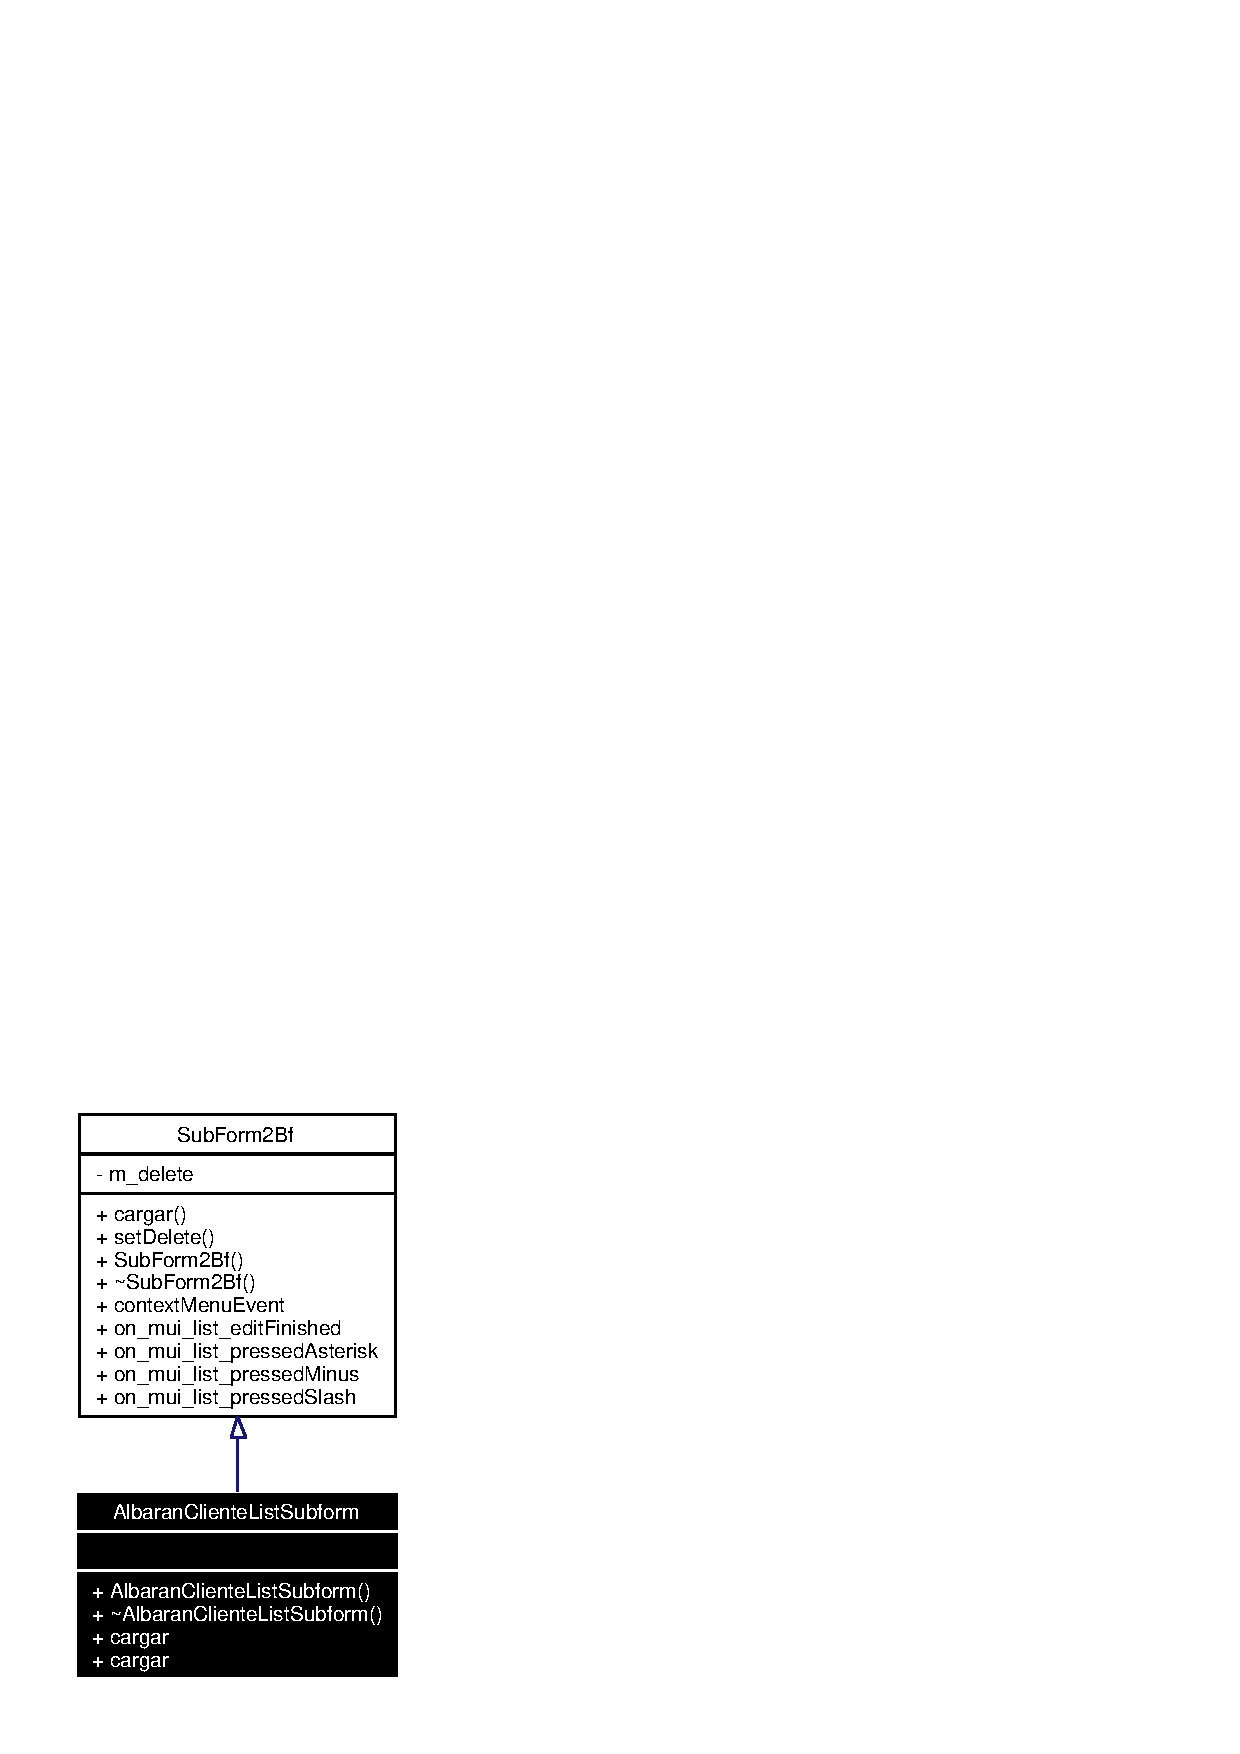
\includegraphics[width=96pt]{classAlbaranClienteListSubform__inherit__graph}
\end{center}
\end{figure}
Diagrama de colaboraci\'{o}n para Albaran\-Cliente\-List\-Subform:\begin{figure}[H]
\begin{center}
\leavevmode
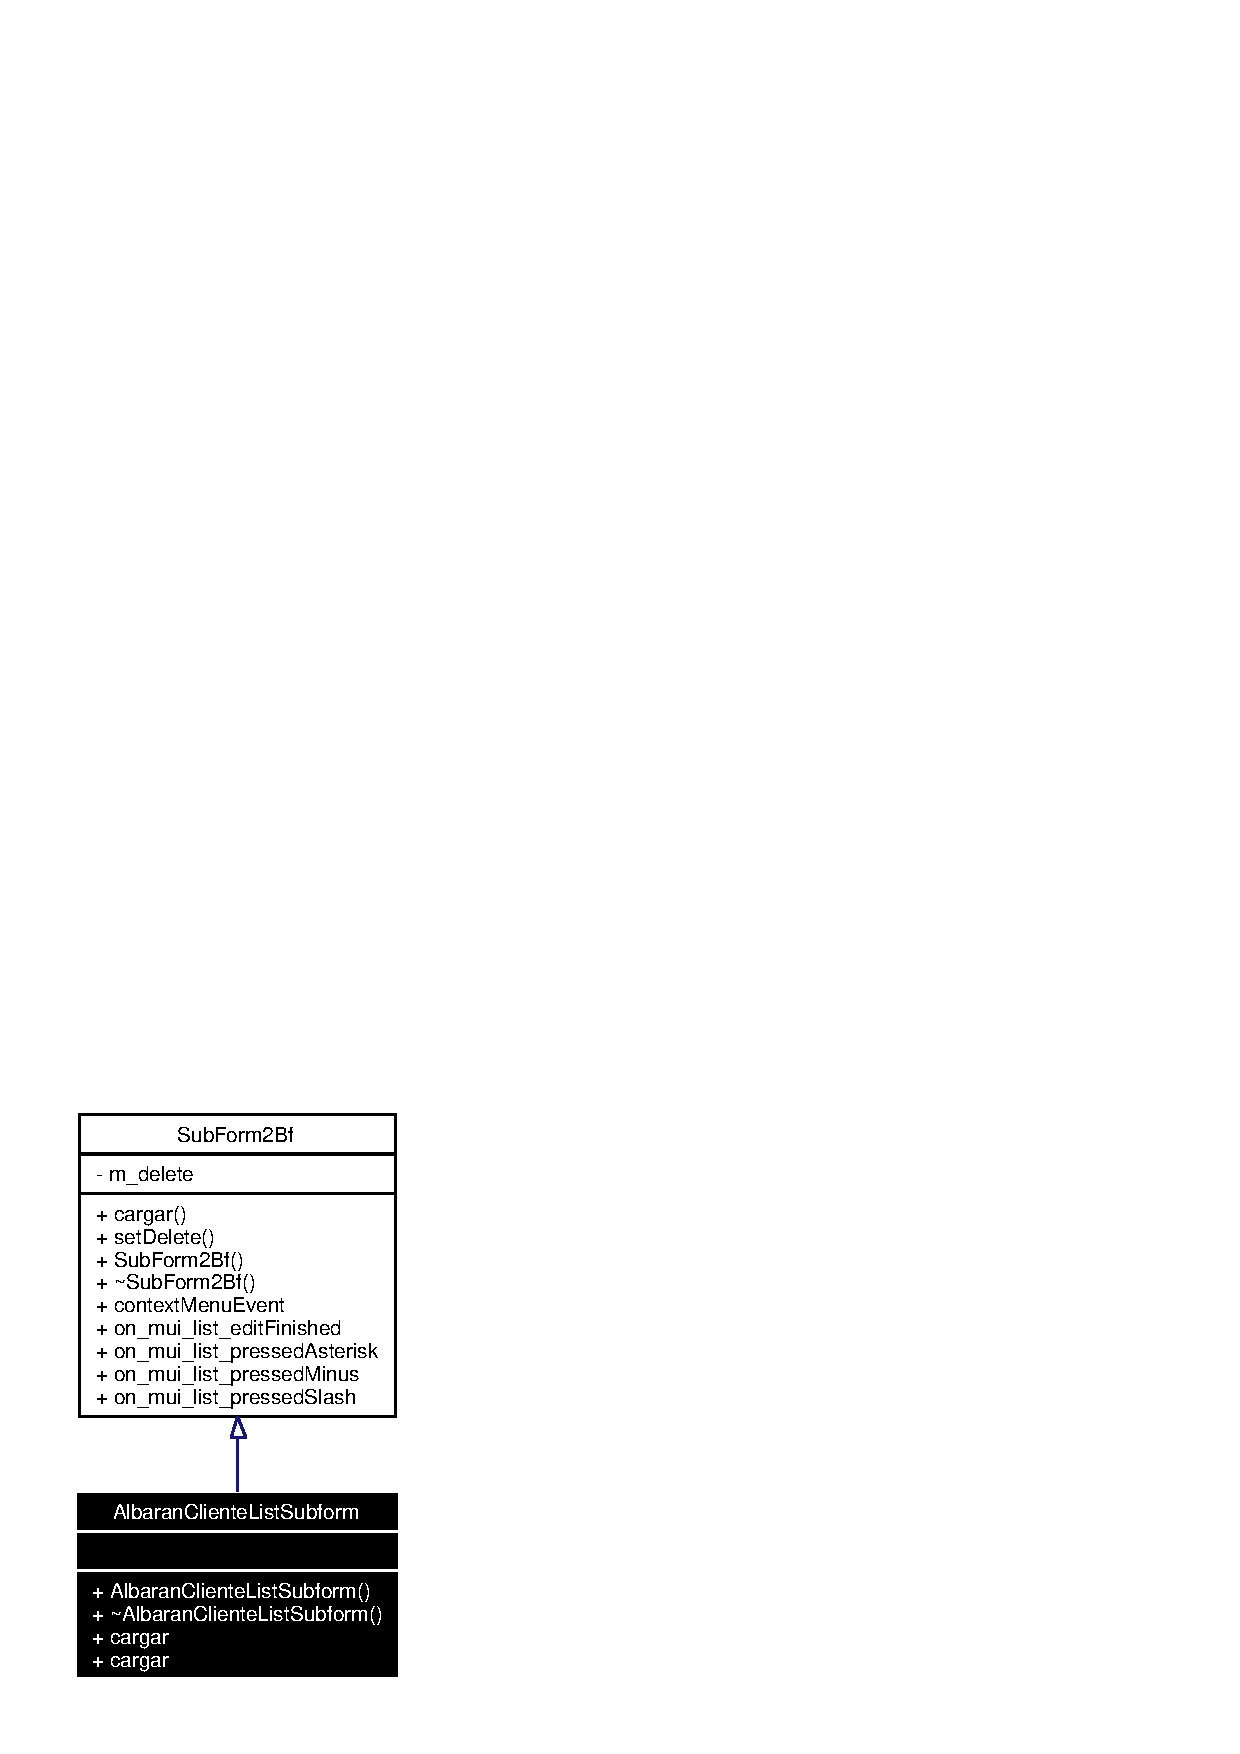
\includegraphics[width=96pt]{classAlbaranClienteListSubform__coll__graph}
\end{center}
\end{figure}
\subsection*{Slots p\'{u}blicos}
\begin{CompactItemize}
\item 
virtual void {\bf cargar} (QString query)\label{classAlbaranClienteListSubform_i0}

\item 
virtual void {\bf cargar} ()\label{classAlbaranClienteListSubform_i1}

\end{CompactItemize}
\subsection*{M\'{e}todos p\'{u}blicos}
\begin{CompactItemize}
\item 
{\bf Albaran\-Cliente\-List\-Subform} (QWidget $\ast$parent=0)
\end{CompactItemize}


\subsection{Descripci\'{o}n detallada}
Listado de albaranes de clientes. 



\subsection{Documentaci\'{o}n del constructor y destructor}
\index{AlbaranClienteListSubform@{Albaran\-Cliente\-List\-Subform}!AlbaranClienteListSubform@{AlbaranClienteListSubform}}
\index{AlbaranClienteListSubform@{AlbaranClienteListSubform}!AlbaranClienteListSubform@{Albaran\-Cliente\-List\-Subform}}
\subsubsection{\setlength{\rightskip}{0pt plus 5cm}Albaran\-Cliente\-List\-Subform::Albaran\-Cliente\-List\-Subform (QWidget $\ast$ {\em parent} = {\tt 0})}\label{classAlbaranClienteListSubform_a0}


============================================================================= SUBFORMULARIO ============================================================================= 

La documentaci\'{o}n para esta clase fu\'{e} generada a partir de los siguientes archivos:\begin{CompactItemize}
\item 
albaranclientelist.h\item 
albaranclientelist.cpp\end{CompactItemize}
